\section{The RDMA-based \paxos Protocol} \label{sec:input}

This section presents \xxx's consensus protocol with its runtime system, 
including the RDMA-based consensus algorithm in normal case 
(\S\ref{sec:normal}), handling concurrent connections (\S\ref{sec:concurrent}), 
leader election (\S\ref{sec:election}), and reliability guarantees 
(\S\ref{sec:guarantees}).

\subsection{Normal Case Algorithm} \label{sec:normal}



% \subsubsection{The Basic } \label{sec:primitive}

% Question: What if on a machine, it viewed it as the leader, it executes the 
% actual socket call, and then it invokes the consensus, but then it is no 
% longer the leader any more. How to undo the actual socket calls? Cases:
  %% On accept(). The old leader has already accepted and asks for consensus.
  %% On recv(). The old leader has already received.
  %% On send().
  %% On close().

% First, basic roles. log format details.
\xxx' input consensus protocol contains three roles (\S\ref{sec:overview}). 
First, the \paxos consensus log. Second, a server program thread on the leader 
replica (in short, a leader thread) which invokes a consensus request. For 
efficiency, \xxx lets leader threads concurrently invoke consensus requests 
when they call inbound socket calls (\eg, \recv). Third, a backup's 
\xxx internal follower thread (\S\ref{sec:overview}) which processes 
consensus requests.

\begin{figure}[h]
\vspace{-.2in}
\centering
\begin{minipage}{.5\textwidth}
\lgrindfile{code/logentry.cpp}
\end{minipage}
\vspace{-.05in}
\caption{{\em \xxx's log entry for each socket call.}} \label{fig:logentry}
\vspace{-.1in}
\end{figure}

Figure~\ref{fig:logentry} shows the format of a log entry in \xxx's consensus 
log. Most fields are regular as those in a typical \paxos 
protocol~\cite{paxos:practical} except three ones: the \v{reply} array, the 
client connection ID \v{conn\_vs}, and the type ID of a socket call 
\v{call\_type}. The \v{reply} array is for backups to WRITE their consensus 
replies to the leader. The \v{conn\_vs} is for identifying which connection this 
socket call belongs to (see \ref{sec:concurrent}). The \v{call\_type} 
identifies four types of socket calls in \xxx: the \accept type (\eg, \accept), 
the \recv type (\eg, \recv and \myread), the \send type (\eg, \send), and the 
\close type (\eg, \close).

% Second, leader thread behavior on \recv(). Return from orig recv, grab 
% spin % lock and get view stamp, store the log, and post send to all replicas. 
% Non blocking. Wait % for over half agree, and then execute the operation.
Figure~\ref{fig:consensus} shows the input consensus algorithm. Suppose a 
leader thread invokes a consensus request when it calls a socket call with the 
\recv type. A consensus request includes four steps. The first step 
(\textbf{L1}) is executing the actual Libc socket call, because \xxx needs to 
get the actual return values or received data bytes of this call and then 
replicates them in remote replicas' logs.

The second step (\textbf{L2}) is local preparation, including assigning a 
global viewstamp to locate this entry in the consensus log, building a log 
entry structure for this call, and writing this entry to a local fast
storage (\S\ref{sec:logging}). 
% without allowing gaps (\ig, newer 
% entries reach consensus but ).

Third, each leader thread concurrently invokes a consensus via the third step 
(\textbf{L3}): WRITE the log entry to remote backups. This step is thread-safe 
because each leader thread works on its own entry and backups' corresponding 
remote entries. An \textbf{L3} WRITE immediately returns after copying the entry 
to its local QP between the leader and each backup. In our evaluation, copying 
a log entry to local QP took 
no more than 0.2 \us. Therefore, the WRITEs to all backups are done almost in 
parallel (all \textbf{L3} arrows in Figure~\ref{fig:logentry}).
% , because \paxos has handled the reliability 
% issues (\eg, packet losses) for our WRITEs


% Instead, \xxx's leader thread just return 
% immediately after 
% putting the structs to the RDMA QP (Queue Pair) between a backup replica, 
% because \paxos protocol \xxx implements has already considered packet losses 
% (\eg, due to remote replica failures).

The fourth step (\textbf{L4}) is the leader thread polling on its \v{reply} 
field in its local log entry for backups' consensus replies. Once consensus is 
reached, the leader thread finishes intercepting this \recv socket call and 
continues with its server application logic.

% 
% The leader does a
% busy loop to check the \v{ack} array until it sees that a majority of replicas, 
% including itself, have aggreed on this log entry. In normal case, both the 
% third and fourth steps will return immediately because no synchronization 
% context switch is involved.

% Post send carry the last committed (consensus reached) operation.

% One key issue, check integrity. Strawmen approach, check viewstamp first.
On a backup side, one tricky synchronization issue is that an efficient way is 
needed to make the leader's RDMA WRITEs and backups' polls atomic. For instance, 
while a leader thread is doing a WRITE on \v{vs} to a remote backup, the
backup's follower thread may be reading \v{vs} concurrently, causing a 
corrupted read value.

To address this issue, one existing approach~\cite{farm:nsdi14,herd:sigcomm14} 
leverages the left-to-right ordering of RDMA WRITEs and puts a special 
non-zero variable at the end of a fix-sized log entry because they mainly 
handle key-value stores with fixed value length. As long as this variable is 
non-zero, the RDMA WRITE ordering guarantees that the log entry WRITE is 
complete. However, because \xxx aims to support general server programs with 
largely variant received data lengths, this approach cannot be applied in \xxx.

Another approach is using atomic primitives provided by RDMA hardware, 
but a prior evaluation~\cite{drtm:sosp15} has shown that RDMA atomic 
primitives are much slower than normal RDMA WRITEs and local memory reads.
% Thus, in a RDMA-accelerated protocol, an extra mechanism 
% is needed to gurantee that a 
% leader's write has finished and then replicas can agree or disagree.

\begin{figure}[t]
\centering
\vspace{-0.4in}
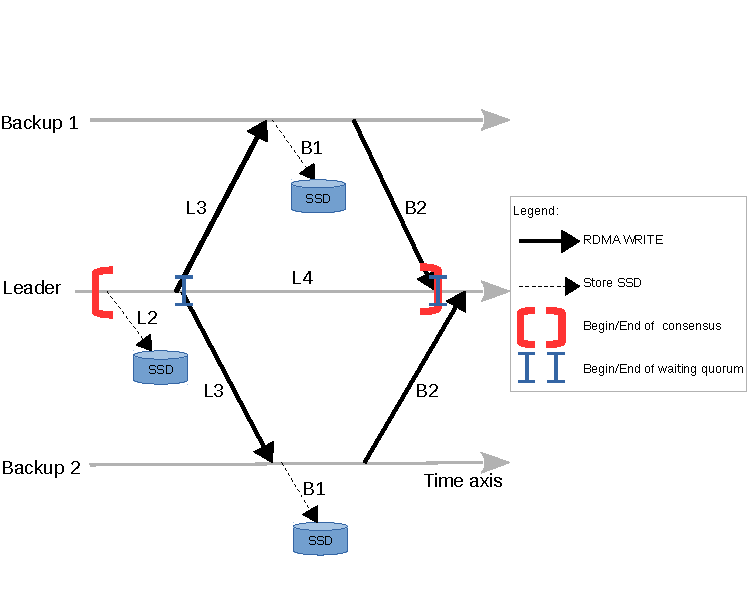
\includegraphics[width=.48\textwidth]{figures/consensus}
\vspace{-.25in}
\caption{{\em \xxx consensus algorithm in normal case.}} \label{fig:consensus}
\vspace{-.2in}
\end{figure}

\xxx tackles this issue by adding a canary value after the actual \v{data} 
array. Because \xxx uses a QP with the type of RC (reliable connection) 
(\S\ref{sec:background}), the follower always first checks the canary value 
according to \v{data\_size} and then starts a standard \paxos consensus reply 
decision~\cite{paxos:practical}. Our efficient, synchronization-free approach 
guarantees that the follower always reads a complete log entry.
% This check guarantees that a log entry is 
% completely written in a local backup.
% 
% To ahchieve small consensus latency, \xxx's follower thread does a busy loop 
% on a dedicated CPU core to agree on consensus requests from the leader. Each 
% backup only needs one follower thread. This thread always busy reading the 
% latest un-agreed log entry in its local log, and it it sees a log entry has 
% completely written, it runs three steps. 

A follower thread in a backup replica polls from the latest un-agreed log 
entry, and it does three steps to agree on consensus requests in order without 
allowing any consensus gaps~\cite{paxos:practical}. First (\textbf{B1}), it 
does a regular \paxos view ID checking to see whether the leader is up-to-date, 
it then stores the log entry in its local SSD. Second (\textbf{B2}), it does a 
WRITE to send back a consensus reply to the leader's \v{reply} array element 
according to its own node ID. Backups perform these two steps in parallel 
(see Figure~\ref{fig:logentry}).

Third (\textbf{B3}, not shown in Figure~\ref{fig:consensus}), the follower 
does a regular \paxos check on \v{last\_committed} and executes all socket 
calls that it has not executed before this viewstamp. It then ``executes" each 
log entry by sending the socket calls to the local server program.
% This 
% forwarding faithfully builds and closes concurrent connections between the 
% follower and the local server program according to the socket calls in the 
% consensus log.
% thus \xxx can 
% maintain consistent concurrent client connection mappings between the leader and 
% backups.


% TBD: should we put the impl here or somewhere else?
% In an implementation level, \xxx stores log entries in local SSD using Berkley 
% DB~\cite{berkeleydb}. Although \xxx's algorithm does not wait every RDMA ACK in 
% order to achieve high scalability, we use selective signaling 
% (\S\ref{sec:background}) to occasionally check and clear ACKs in the CQ 
% associated with the QP, an essential ACK clearing step in RDMA implementations.

% On replicas, server programs run as is without being 
% intercepted. In short, this follower thread runs a high performance loop to 
% respond consensus requests and forward data to the local server program. Since 
% each backup machine only has one follower thread and nowadays machines often 
% have spare cores, we didn't find that the spin loop of this thread brought 
% bring negative performance impact in our evaluation.

% Performance: two RDMA writes and two SSD stores. No context switches.
% This protocol is highly optimized for minimizing consensus latency in normal 
% case. In total, a consensus between the leader and one backup only requires 
% two one-sided RDMA write operations (one from the leader to the backup and the 
% other from the backup to the leader) and two SSD write operations (each in 
% leader and backup). Although each RDMA one-sided operation takes about 3 \us, 
% \xxx's protocol just puts the log entry to the RDMA Queue Pair without needing 
% to wait until the write succeeds on the remote backup, because the leader will 
% have \paxos's consensus reply (the RDMA write from the backup to leader). In 
% addition, neither a leader thread or a follower thread does a synchronization 
% context switch during this consensus (a synchronization context switch 
% typically takes sub milli seconds, pretty slow).

% Question: one key question, can RDMA lose packets in between? I mean, both 
% data_size and canary value are correct, but packets in the middle are lost. 
% This may violate \paxos's non-corrupting packets assumption.

% Third, replica thread behavior on \recv(). Block on latest un agreed log, 
% wait for the % consensus log, check integrity, check view id, and then store to 
% BDB. and % then execute the committed but not executed requests from BDB.

\subsection{Handling Concurrent Connections} \label{sec:concurrent}

Unlike traditional \paxos protocols which mainly handle single-threaded 
programs due to the deterministic state machine assumption in SMR, \xxx aims to 
support both single-threaded as well as multithreaded server programs running 
on multi-core machines. Therefore, a strongly consistent mechanism is needed to 
map every concurrent client connection on the leader and to its corresponding 
connection on backups. A naive approach could be matching a leader connection's 
socket descriptor to the same one on a backup, but backups' servers may return 
nondeterministic descriptors due contentions on systems resources.

Fortunately, \paxos already makes viewstamps~\cite{paxos:practical} of 
socket calls strongly consistent across replicas. For TCP connections, \xxx 
adds the \v{conn\_vs} field, the viewstamp of the the first socket call in 
each connection (\ie, \accept) as the connection ID for log entries. Then, \xxx 
maintains a hash map on each local replica to map this connection ID to local 
socket descriptors.

% On a local 
% replica, \xxx maintains a hash map between this connection ID 
% to the actual local socket descriptor for each connection, then \xxx ensures 
% that data bytes are forwarded from a leader's connection to the right matching 
% connection on backups. \xxx also intercepts socket calls with the \close type 
% to clean up this map. For servers that use UDP to serve requests, \xxx maps the 
% viewstamp of a \recvfrom call to the socket descriptor returned from this call, 
% and it cleans up the map on a corresponding \sendto call. 

% TBD. Strawmen approach, use fds on leader machines.

%% thread ID mapping is not good too, because accept and recv can be called by 
% different threads in leader side.

% Use viewstamp of the accept() operation, consistent across replicas.


% What does replica thread do. High performance loop on a dedicated core.

\subsection{Leader Election} \label{sec:election}

% % Use one log operation or a few operations to do so. Clean, 
% match the PMS intention. Explain why this design choice is good.

% TBD. Four steps. Four entries?
% Compared to traditional \paxos leader election protocols, 
Leader election on RDMA raises a main issue: because backups do 
not communicate frequently with each other in normal case, thus a backup does 
not know the remote memory locations where the other backups are polling. 
Writing to a wrong remote memory location may cause the other backups to miss 
all leader election messages. A recent system~\cite{dare:hpdc15} establishes 
an extra control QP to handle leader election, complicating deployments.

% If current leader fails, 
% how does a backup know the other remote backups' memory location to WRITE to? 

% Mention old leader.
% The second issue still stems from RDMA's nature: while a leader election is 
% on going, the out-dated leader may still WRITE to remote backups and corrupt 
% the ongoing leader election. This WRITE will not get a Yes consensus reply 
% because the other replicas can transit their current state from active to a 
% leader election state~\cite{paxos:practical}, but the old leader's WRITE may 
% still corrupt the ongoing leader election. 

\xxx addresses this issue with a simple, clean design. It runs a leader 
election with the same consensus log and the same QP. In normal case, the 
leader does WRITEs to remote logs as heartbeats with a period of T. Each 
consensus log maintains a control data structure called \v{elect[MAX]}, one 
element for each replica. Normal case operations and heartbeats use the other 
parts of the consensus log but leave this \v{elect} array alone. Once backups 
miss heartbeats from the leader for 3*T, they close the outdated leader's QPs 
and elect a new leader by making follower threads poll the \v{elect} array.

% Before starting a standard leader election 
% phase as in traditional \paxos protocols~\cite{paxos:practical}, each backup 
% always first does RDMA one-sided reads to get remote replicas' current polling 
% location.

Backups start a standard \paxos leader election 
algorithm~\cite{paxos:practical} with three steps. Each replica writes to its 
own \v{elect} element at remote replicas. First, backups propose a new view 
with a standard two-round \paxos consensus~\cite{paxos:simple} by including 
both the view and the index of the latest log entry. The other backups also 
propose their views and poll on this array in order to follow other proposals 
or confirm itself as the winner. The backup whose log is more up-to-date will 
win. A log is more up-to-date if its latest entry has either a higher view or 
the same view but a higher index.

Second, the winner proposes itself as a leader candidate using this 
array, another two-round \paxos consensus. Third, after the second step reaches 
a quorum, the new leader notifies remote replicas itself as the new leader and 
it starts to WRITE periodic heartbeats. Overall, \xxx safely avoids multiple 
``leaders" to corrupt consensus logs, because only one leader is elected in 
each view, and backups always close an outdated leader's QPs before electing a 
new leader.


\subsection{Reliability Guarantee} \label{sec:guarantees}

% Follow PMP, ease to understand, absorbe good exeprience.
% \paxos is notoriously difficult to 
% understand~\cite{raft:usenix14,paxos:simple,paxos,paxos:complex} or 
% implement~\cite{paxos:live,paxos:practical}. 
% 
To minimize protocol-level bugs, \xxx's protocol derives from a viewstamp-based 
protocol~\cite{paxos:practical}. We made this design choice because \paxos is 
notoriously difficult to 
understand~\cite{raft:usenix14,paxos:simple,paxos,paxos:complex}, 
implement~\cite{paxos:live,paxos:practical}, or 
verify~\cite{modist:nsdi09,demeter:sosp11}. Deriving from a viewstamp-based 
protocol~\cite{paxos:practical} helps us incorporate these 
readily mature understanding, engineering experience, and the theoretically 
verified safety rules into our protocol.

% TBD: reliability analyzes. We do not need the lossless assumption in RDMA QPs.
Although \xxx's \paxos protocol works on a RDMA network, the reliability of 
\xxx does not rely on a lossless RDMA (\eg, network devices can fail). \xxx 
still provides same fault-tolerance guarantee as the standard \paxos model, 
where a stable storage exists, but replicas may fail, and server programs may 
crash.


% Define safety: TBD.
% A \paxos protocol must ensure safety: the agreed operation must be an actually 
% proposed one; if agreed, all active replicas must consistently enforce this 
% operation. Safety is another important sweet spot that \xxx's input 
% coordination protocol inherites from traditional \paxos protocol by sticking 
% with same replica behavior in traditional ones. As a traditional protocol, 
% our input coordination protocol also uses view IDs and viewstamps to enforce a 
% consistent, up-to-date leadership across replicas. To address the atomicy issue 
% between remote RDMA writes and local memory reads, our protocol addes an 
% completion check on log entries (\S\ref{sec:normal}).
% In short, our 
% design choice makes our input coordination protocol enforce the same level of 
% safety as traditional \paxos protocols~\cite{paxos, paxos:simple, 
% paxos:practical}.

% Safety, viewstamp.

% Store to stable storage.

% Any unique changes that prevent us from providing guarantees? The delta 
% changes? Packets. Logs?

% \begin{figure}[t]
% \centering
% \vspace{-.20in}
% 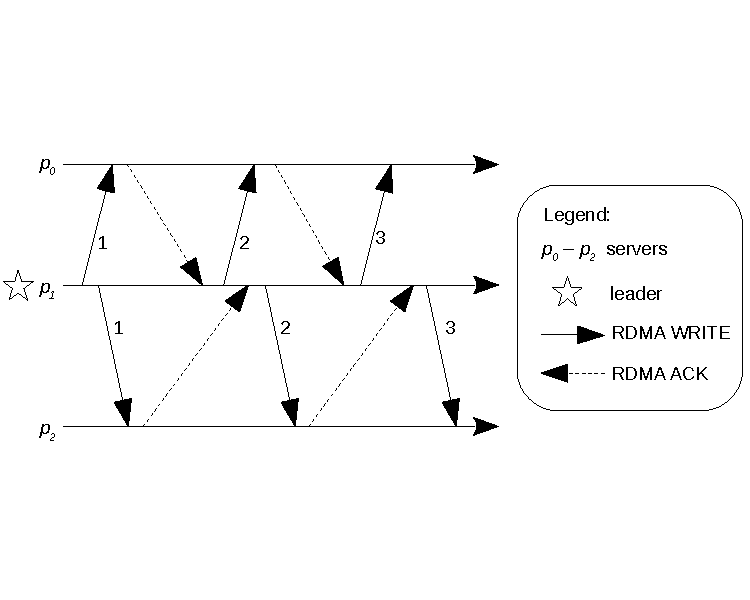
\includegraphics[width=.48\textwidth]{figures/dare}
% \vspace{-.20in}
% \caption{{\em DARE consensus algorithm in normal case.}} \label{fig:dare}
% \vspace{-.05in}
% \end{figure}
% 
% We compare the performance and scalability between \xxx and DARE, the fastest 
% RDMA-based consensus algorithm we know so far. As shown on 
% Figure~\ref{fig:consensus}, a complete \xxx consensus round consists of three 
% parts: a leader's local SSD store operation (L2), a backup's local SSD store 
% operation (B1), and a WRITE round-trip (L3 and B2). Given the same inputs, 
% the latency of these three parts are constant, thus \xxx's consensus latency is 
% not approximately constant to replica group size. \xxx's scalability is mainly 
% bounded by the max number of outbound RDMA writes in the RDMA NIC hardware 
% (currently, 16~\cite{herd:sigcomm}).
% 
% We carefully examined DARE's code base and depict its consensus algorithm in 
% Figure~\ref{fig:dare}, which consists of three parts: log entry WRITEs to all 
% remote logs' with ACKs, log tail pointer WRITEs to all remote logs with ACKs, 
% and a quorum notification by WRITEs to agreed remote replicas without ACKs. In 
% DARE's pure leader-based consensus, ACKs are necessary for every next step to 
% start. Therefore, DARE's consensus latency is linear to replica group size. We 
% show concrete consensus latency comparisons of \xxx and DARE in evaluation 
% (\S\ref{sec:scalability}).